%-------------------------
%big-picture
%(c) H.Buchmann FHNW 2008
%$Id$
%export TEXINPUTS=${HOME}/fhnw/edu/:${HOME}/fhnw/edu/tinL/config/latex:${HOME}/fhnw/edu/config//:
%-------------------------
\documentclass{beamer}
\usepackage{latex/beamer}
%---------------------
%local defines
%(c) H.Buchmann FHNW 2009
%$Id$
%---------------------
\newcommand{\target} {\beaglebone\xspace}
\newcommand{\targetS}{{\bf BBG}\xspace}
\newcommand{\host}   {{\em Host}\xspace}
\newcommand{\targetroot} {{\bf target-root}\xspace}
\newcommand{\kernel} {{\bf kernel}\xspace}
\renewcommand{\c}{{\bf C}\xspace}
\newcommand{\cpp}{{\bf C++}\xspace}
\newcommand{\posix}{{\bf POSIX}\xspace}


\title{Image auf SD Karte}
\begin{document}

\newcommand{\distro}{sd-2016-09-28.img.gz}

\frame{\titlepage}

\begin{frame}{Ziel}{Image auf SD-Karte}
 \begin{itemize}
  \item Wie startet ein Rechner
  \begin{itemize}
   \item booten
  \end{itemize}
  \item Partitionen
  \begin{itemize}
   \item alles ist ein File
  \end{itemize}
  \item die serielle Schnittstelle via USB
  \begin{itemize}
   \item der erste Kontakt mit dem \target
  \end{itemize}
  \item Image
  \begin{itemize}
   \item per USB am lokalen Netz \host - \targetS
   \item per Wi-Fi am Internet
  \end{itemize}
 \end{itemize}
\end{frame}

%-------------------------
%minimal-unix
%(c) H.Buchmann FHNW 2014
%export TEXINPUTS=.:${HOME}/fhnw/edu/:${HOME}/fhnw/edu/tinL/config/latex:${HOME}/fhnw/edu/config//:
%-------------------------
\documentclass{beamer}
\usepackage{latex/beamer}
%---------------------
%local defines
%(c) H.Buchmann FHNW 2009
%$Id$
%---------------------
\newcommand{\target} {\beaglebone\xspace}
\newcommand{\targetS}{{\bf BBG}\xspace}
\newcommand{\host}   {{\em Host}\xspace}
\newcommand{\targetroot} {{\bf target-root}\xspace}
\newcommand{\kernel} {{\bf kernel}\xspace}
\renewcommand{\c}{{\bf C}\xspace}
\newcommand{\cpp}{{\bf C++}\xspace}
\newcommand{\posix}{{\bf POSIX}\xspace}

\input{/home/buchmann/latex/dirtree/dirtree.tex}

\usepackage[absolute]{textpos}
\setlength{\TPHorizModule}{1mm}
\setlength{\TPVertModule}{1mm}

\begin{document}

\newcommand{\md}{\cod{md-bbb-{\em version}.img}}
\newcommand{\mdev}{\cod{md-bbb-devel-{\em version}.tar.gz}}
\title[Boot]{Boot\\die verschiedenen M�glichkeiten}

\frame{\titlepage}

\begin{frame}{\target} {Die Boot Devices}
  \begin{description}
   \item[SPI0] {\bf S}erial {\bf P}eripheral {\bf I}nterface
   \item[MMC1] die eingebaute SD-Card
   \item[MMC0] die externe SD-Card
   \item[UART0] die serielle Schnittstelle
   \item[USB0] USB Schnittstelle
  \end{description}
\end{frame}

\begin{frame}{\target}{zwei M�glichkeiten}
\begin{columns}
\begin{column}{0.5\textwidth}
 \begin{itemize}
  \item die normale:
   \begin{itemize}
    \item \cod{MMC1}, \cod{MMC0}, \cod{UART0}, \cod{USB0}
   \end{itemize}
   \item Boot Switch
   \begin{itemize}
    \item \cod{SPI0}, \cod{MMC0}, \cod{USB0}, \cod{UART0}
   \end{itemize}
 \end{itemize}
\end{column}
\begin{column}{0.5\textwidth}
 \includegraphics[width=0.75\textwidth]{bbb-boot.pdf}
\end{column}
\end{columns} 
\end{frame}

\end{document}

\section{Partitionen}
\begin{frame}{Partition}
 \begin{itemize}
  \item Träger von Filesystemen
  \item Aufbau
  \begin{itemize}
   \item MBR: Master Boot Record
  \end{itemize}
  \item Herstellung
 \end{itemize}
 \remark{Alles ist ein File  {\em stream of bits}}
\end{frame}

\subsection{Massenspeicher}
\begin{frame}{Massenspeicher}{non volatile}
 \begin{block}{Arten}
  \begin{itemize}
   \item mechanische Festplatten
   \item SSD Karten
   \item SD-Karten
   \item Flash
   \item ...
  \end{itemize}
 \end{block}
 \begin{block}{Typisch}
  \begin{itemize}
   \item Zugriff relativ langsam
   \item Blockorientiert 
   \begin{itemize}
    \item Mehrere Bits/Bytespro Zugriff
   \end{itemize}
  \end{itemize}
 \end{block}
\end{frame}


\begin{frame}{Partitionen Termiologie \linux}{Träger von Filesystemen}
  \begin{itemize}
   \item Massenspeicher
   \begin{itemize}
   \item \cod{/dev/sd{\em X}}, \cod{{\em X}=a,b,c ...}
   \end{itemize} 
   \item Partitionen 
   \begin{itemize}
     \item \cod{/dev/sd{\em X}{\em N}} \cod{{\em N}=1,2,3 ...} 
   \end{itemize} 
  \end{itemize}
  \begin{block}{\Huge Vorsicht}
   \begin{itemize}
    \item Festplatte vom \host ist auch ein \cod{/dev/sd{\em X}}
   \end{itemize}
  \end{block}
\end{frame} 


\begin{frame}[fragile]{Massenspeicher}{Blocks/Sektoren}
\begin{lstlisting}
 typedef unsigned char Sector[512]; 
 Sector MassStorage[N];
\end{lstlisting}
\remark{Ein langer Array von Sektoren}
\begin{center}
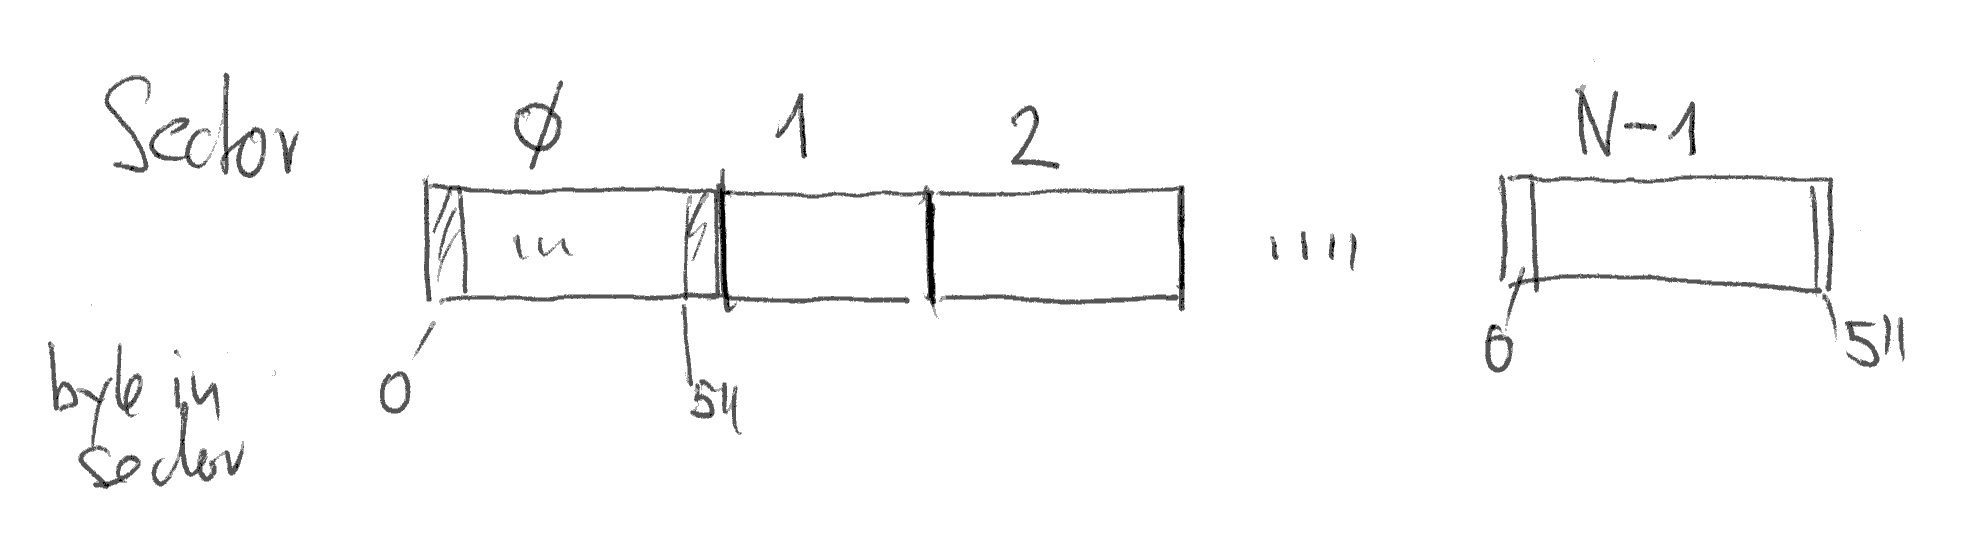
\includegraphics[width=0.875\textwidth]{array-of-sector.jpg}
\end{center}
\end{frame}

\begin{frame}[fragile]{Der Befehl \cod{dd}}{Vorsicht}
\begin{lstlisting}[language=bash]
dd if=/dev/sdX count=1|hexdump -C        
  # first sector to stdout
dd if=/dev/sdX skip=1 count=1|hexdump -C 
  # second sector to stdout
dd if=/dev/sdX of=mbr.bin count=1        
  # copy sector to mbr.bin
\end{lstlisting}
  \begin{block}{\Huge Vorsicht}
   \begin{itemize}
    \item Festplatte vom \host ist auch ein \cod{/dev/sd{\em X}}
   \end{itemize}
  \end{block}

\end{frame}

\subsection{MBR}
\begin{frame}[fragile]{MBR: Master Boot Record}{Verzeichnis der Partionen}
\begin{lstlisting}[language=bash]
dd if=/dev/mmcblk0 count=1|hexdump -C
\end{lstlisting}
{\scriptsize
\begin{verbatim}
00000000  00 00 00 00 00 00 00 00  00 00 00 00 00 00 00 00  |................|
*
000001b0  00 00 00 00 00 00 00 00  ba 23 8e d6 00 00 00 00  |.........#......|
000001c0  01 20 0b 03 10 1f 00 08  00 00 00 00 04 00 00 00  |. ..............|
000001d0  01 20 83 03 50 df 00 08  04 00 00 70 71 00 00 00  |. ..P......pq...|
000001e0  00 00 00 00 00 00 00 00  00 00 00 00 00 00 00 00  |................|
000001f0  00 00 00 00 00 00 00 00  00 00 00 00 00 00 55 aa  |..............U.|
00000200
\end{verbatim}
}

{\scriptsize\url{technet.microsoft.com/en-us/library/cc976786.aspx}}

\end{frame}


\section{Serielle Schnittstelle}
\begin{frame}{USB-Serial}
\begin{columns}
\begin{column}{0.5\textwidth}
\includegraphics[height=0.825\textheight]{pin.pdf}
\end{column}
\begin{column}{0.5\textwidth}
\begin{block}{Cable}
\vspace{5mm}
\begin{tabular}{c|c}
Color & Signal\\
\hline
BLACK & GND\\
GREEN & TX\\
WHITE & RX
\end{tabular}
\end{block}
\end{column}
\end{columns}
\end{frame}



\section{SD Karte}
\begin{frame}{Initiale SD-Karte}{Herstellung}
 \begin{itemize}
  \item das Image:
  \begin{itemize}
   \item \href{https://drive.switch.ch/index.php/s/VDDlivnHq2QQ8m9}{sd-2019-09-26.img.xz}
  \end{itemize}
  \item auf SD-Karte
  \begin{itemize}
   \item \cod{xz -d -c sd-2020-03-04.img.xz | sudo dd of=/dev/sdX}
   \begin{remarks}
   \item {\Huge Vorsicht} bei \cod{/dev/sdX}
   \item File \cod{sd-2020-03-04.img.xz} im \href{https://drive.switch.ch/index.php/s/A6H382zEGDrgfAL}
                      {\color{red}$\to$Verzeichnis}
   \end{remarks}
  \end{itemize}
 \end{itemize}
\end{frame}

\begin{frame}[fragile]{2 Partitionen}{gemacht mit \cod{fdisk -l /dev/sdX}}
{
\footnotesize
\begin{verbatim}
Disk /dev/sda: 14.5 GiB, 15552479232 bytes, 30375936 sectors
Disk model: STORAGE DEVICE  
Units: sectors of 1 * 512 = 512 bytes
Sector size (logical/physical): 512 bytes / 512 bytes
I/O size (minimum/optimal): 512 bytes / 512 bytes
Disklabel type: dos
Disk identifier: 0x00000000

Device     Boot Start    End Sectors  Size Id Type
/dev/sda1  *     2048  34815   32768   16M  b W95 FAT32
/dev/sda2       34816 559103  524288  256M 83 Linux
\end{verbatim}
}
\begin{description}
 \item[p1] Boot Partition
 \item[p2] Root Filesystem das Linux
\end{description}
\end{frame}

%\subsection{Distribution}
%\begin{frame}[fragile]{Alles ist ein File}{und umgekehrt}
%\begin{itemize}
% \item Der File \cod{\distro}
% ist das Bild einer ganzen SD-Karte
% \item Mache SD-Karte
% \begin{itemize}
%  \item Kopiere {\tiny\url{sourceforge.net/projects/fhnw-tinl/files/{\distro}/download}} 
%  \item entzippe
%  \item kopiere
%  \begin{lstlisting}
%dd if=distro.img of=/dev/sd-card
%  \end{lstlisting}
%  \cod{sd-card} typ \cod{mmcblk\em{N}} $N=0|1 ..$
% \end{itemize}
% \remark{Alles mit {\em pipes}}
% 
%\end{itemize}
%
%\end{frame}

\end{document}

